%====================================================%
% SEZIONE 1: Definizione
%====================================================%
\begin{question}[ID=1.1, subtitle={Riconoscimento di funzioni esponenziali}, difficulty=facile, tags={definizione, esponenziali}]
Descrivere quali fra le seguenti funzioni sono esponenziali e spiegare il motivo
\begin{center}\begin{minipage}{0.92\linewidth}
\begin{multicols}{2}
\begin{enumerate}[leftmargin=3.2cm]
\item $y=3^{-x}$
\item $y=(-2)^x$
\item $y=0{,}5^{2x}$
\item $y=(\sqrt{3})^x$
\end{enumerate}
\end{multicols}
\end{minipage}\end{center}
\begin{solution}Sono esponenziali: $a)$ $y=3^{-x}$ (base $>0$, $\neq1$); $c)$ $y=0{,}5^{2x}$ (base $>0$, $\neq1$); $d)$ $y=(\sqrt{3})^x$ (base $>0$, $\neq1$). Non è esponenziale $b)$ perché la base è negativa.\end{solution}
\end{question}

%----------------------------------------------------%

%====================================================%
% SEZIONE 2: Grafici
%====================================================%
\begin{question}[ID=2.1, subtitle={Associazione tra funzioni esponenziali e grafici}, difficulty=facile, tags={grafici, esponenziali}]
Associare a ogni funzione il grafico corretto:
\begin{center}\begin{minipage}{0.92\linewidth}
\begin{multicols}{2}
\begin{enumerate}[label=\arabic*),leftmargin=2cm]
\item $y=\Big(\dfrac{3}{2}\Big)^x$
\item $y=\Big(\dfrac{1}{2}\Big)^x$
\item $y=4^{x}$
\item $y=\Big(\dfrac{1}{3}\Big)^{\frac{x}{2}}$
\end{enumerate}
\end{multicols}
\end{minipage}\end{center}

\begin{center}
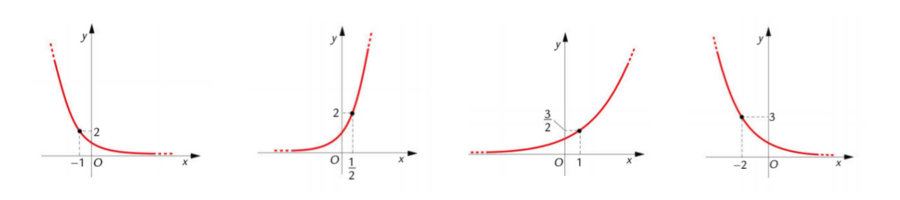
\includegraphics[width=\textwidth]{images/grafici_esponenziali.png}
\end{center}
\vspace{-30pt}
\[ \text{a)} \hspace{30pt} \text{b)} \hspace{30pt} \text{c)} \hspace{30pt} \text{d)} \]
\begin{solution}
Tutti i grafici passano per $(0,1)$. Si distinguono con due criteri: \emph{monotonia} (base $>1$ crescente, base $<1$ decrescente) e \emph{ripidità} (tanto più la base è lontana da $1$, tanto più la curva è ripida).
\begin{itemize}
\item 1) $\big(\tfrac32\big)^x$: base $>1$, \textbf{crescente} ma poco ripida.
\item 2) $\big(\tfrac12\big)^x$: base $<1$, \textbf{decrescente} e ripida.
\item 3) $4^x$: base $>1$, \textbf{crescente} e molto ripida (la più ripida tra le crescenti).
\item 4) $\big(\tfrac13\big)^{x/2}=\big(\tfrac{1}{\sqrt3}\big)^x\approx(0{,}577)^x$: base $<1$, \textbf{decrescente} e meno ripida della 2).
\end{itemize}
Si associa quindi: le crescenti (1 e 3) ai due grafici che salgono, distinguendole per pendenza (3 più ripida di 1); le decrescenti (2 e 4) ai due che scendono (2 più ripida di 4).
\end{solution}
\end{question}

%====================================================%
% SEZIONE 3: Equazioni
%====================================================%
\begin{question}[ID=3.1, subtitle={Equazioni esponenziali elementari}, difficulty=facile, tags={equazioni, esponenziali}]
Calcolare il valore di $x$ nelle seguenti equazioni:
\begin{center}\begin{minipage}{0.92\linewidth}
\begin{multicols}{2}
\begin{enumerate}[leftmargin=3.2cm]
\item $3^{x} = 81$
\item $2^{x+1} = 4 \color{gray}$
\item $\color{gray}\dfrac{9}{3^x} = 27$
\item $e^{2x-1} = \dfrac{1}{e^2}$
\item $25 \cdot 5^{2x} = \dfrac{1}{5} \cdot 5^{x-1}$
\item $9^{-x} = -3$
\item $2^{2x} - 2^{x+2} + 4 = 0 \color{gray}$
\item $\color{gray} 5^{2x} + 3 \cdot 5^x + 2 = 0$
\end{enumerate}
\end{multicols}
\end{minipage}\end{center}
\begin{solution}$a)\ x=4$; $b)\ x=1$; $c)\ x=-1$; $d)\ x=-\tfrac{1}{2}$; $e)\ x=-2$; $f)$ impossibile; $g)\ x=1$\end{solution}
\end{question}
